\lstinputlisting[language=bash,basicstyle=\small]{python_codes/fieldstone_57/keywords.ascii}

\begin{center}
Code at \url{https://github.com/cedrict/fieldstone/tree/master/python_codes/fieldstone_57}
\end{center}

\par\noindent\rule{\textwidth}{0.4pt}

{\sl This stone was developed in collaboration with Jort Jansen}. \index{contributors}{J. Jansen}

\par\noindent\rule{\textwidth}{0.4pt}

%%%%%%%%%%%%%%%%%%%%%%%%%%%%%%%%%%%%%%%%%%%%%%%%%%%%%%%%%%%%%%%%%%%%%%%%%%%%%%%%%%%%%%%%%%%%%

Boundary conditions are $T(x=0)=0$ and $T(x=1)=1$. All material coefficients are set to 1
so that we are solving $d^2T/dx^2=0$ over the domain $[0,1]$. The analytical solution is 
of course $T(x)=x$ and $q(x)=1$ (Note that because of the conventions used in the book 
we used $q$ is here positive!). 

%-----------------------------------------------------------------------------------------
\subsubsection*{The code}

We follow the discretisation presented in Section~\ref{ss:dgss1D} and use the 
successive substitution to arrive at the solution. 

There are {\tt nelx} linear elements and therefore {\tt nnx} nodes.
We start by generating an array containing the coordinates of the nodes:
\begin{lstlisting}
x=np.linspace(0,Lx,nnx)
\end{lstlisting}
We then need to declare arrays for temperature and heat flux, both on the left and on the right of 
each node:
\begin{lstlisting}
T_min=np.zeros(nnx,dtype=np.float64)       
T_plus=np.zeros(nnx,dtype=np.float64)      
q_min=np.zeros(nnx,dtype=np.float64)       
q_plus=np.zeros(nnx,dtype=np.float64)
\end{lstlisting}
and we will need the corresponding arrays keeping track of their previous values:
\begin{lstlisting}
T_min_old=np.zeros(nnx,dtype=np.float64)    
T_plus_old=np.zeros(nnx,dtype=np.float64)   
q_min_old=np.zeros(nnx,dtype=np.float64)    
q_plus_old=np.zeros(nnx,dtype=np.float64)
\end{lstlisting}

The boundary condition at $x=0$ is imposed by setting
\begin{lstlisting}
T_min[0]=T_left
\end{lstlisting}
while the boundary condition at $x=L_x$ is imposed by setting
\begin{lstlisting}
T_plus[nnx-1]=T_right
\end{lstlisting}

Because the element size $h_x$ is constant we can precompute the three required matrices:
\begin{lstlisting}
K=np.array([[hx/3,hx/6,-C ,-0.5],
            [hx/6,hx/3,0.5,-C  ],
            [C   ,-0.5,E  ,0   ],
            [0.5 ,C   ,0  ,E   ]])
\end{lstlisting}
which corresponds to the matrix of Eq.~\eqref{eq:dgsyst1D},
\begin{lstlisting}
K_left=np.array([[hx/3,hx/6,-0.5,-0.5],
                 [hx/6,hx/3, 0.5,-C  ],
                 [0.5 ,-0.5, E  ,0   ],
                 [0.5 ,C   , 0  ,E   ]])
\end{lstlisting}
which corresponds to the matric of of Eq.~\eqref{eq:dgsyst1Dleft},
\begin{lstlisting}
K_right=np.array([[hx/3,hx/6,-C ,-0.5],
                  [hx/6,hx/3,0.5,0.5 ],
                  [C   ,-0.5,E  ,0   ],
                  [0.5 ,-0.5,0  ,E   ]])
\end{lstlisting}
which corresponds to the matrix of Eq.~\eqref{eq:dgsyst1Dright}.
 
We then start iterating
\begin{lstlisting}
for it in range(0,niter):
\end{lstlisting}
and update the flux at the boundaries:
\begin{lstlisting}
q_min[0]     =q_plus[0]   -E*(T_min[0]    -T_plus[0])     # left boundary
q_plus[nnx-1]=q_min[nnx-1]-E*(T_min[nnx-1]-T_plus[nnx-1]) # right boundary
\end{lstlisting}
We then need to loop over all elements, of each we find the corresponding
value for $k$ ({\tt k}) and $k+1$ ({\tt kp1}).
If the loop index points at the first element ({\tt iel==0})
then the matrix ${\bm K}_{el}$ is ${\bm K}_{left}$, 
if the loop index points at the last element ({\tt iel==nel-1})
then the matrix ${\bm K}_{el}$ is ${\bm K}_{right}$, 
otherwise ${\bm K}_{el}$ is ${\bm K}$ from Eq.\eqref{eq:dgsyst1D}.

In all three cases the rhs vector {\tt rhs\_el} is filled according to 
Eqs.~\eqref{eq:dgsyst1Dleft}, \eqref{eq:dgsyst1Dright} and \eqref{eq:dgsyst1D} respectively.

When the elemental matrix and rhs are established for the element under consideration
then the systen is solved and $q_k^+$, $q_{k+1}^-$, $T_k^+$ and $T_{k+1}^-$ are updated.

The iteration loop continues until convergence has been reached, i.e.
when the difference between the new $T$, $q$ at all points and the previous
values is smaller than the chosen tolerance. 

Finally, still inside the iteration loop we must transfer the newly obtained values to the 
'old' arrays:
\begin{lstlisting}
T_min_old[:] =T_min[:]
T_plus_old[:]=T_plus[:]
q_min_old[:] =q_min[:]
q_plus_old[:]=q_plus[:]
\end{lstlisting}



%-----------------------------------------------------------------------------------------
\subsubsection*{Results}

Let us start by fixing ${\cal E}=4$ and ${\cal C}=0$ and setting the absolute convergence 
tolerance to $10^{-8}$. The code converges after 220 iterations and we indeed recover the 
expected temperature and heat flux fields:

\begin{center}
\includegraphics[width=8cm]{python_codes/fieldstone_57/results/E04_C000/convergence.pdf}
\end{center}

\begin{center}
\includegraphics[width=8cm]{python_codes/fieldstone_57/results/E04_C000/T_minus_evol.pdf}
\includegraphics[width=8cm]{python_codes/fieldstone_57/results/E04_C000/q_minus_evol.pdf}
\end{center}

%...................................................
\paragraph{Effect of resolution} Keeping the same parameters we see that the 
number of required iterations to convergence increases linearly with the number of elements.

\begin{center}
\begin{tabular}{cc}
\hline
nelx & \# iterations \\
\hline
08 &60  \\
16 &116 \\
32 &220 \\
64 &436 \\
128 & 857 \\
\hline
\end{tabular}
\end{center}

%...................................................
\paragraph{Effect of ${\cal E}$ \& ${\cal C}$ values} 
We now keep nelx=32 and explore the effect of these parameters on the 
required number of iterations:

\begin{center}
\begin{tabular}{ccc}
\hline
${\cal E}$ & ${\cal C}$ & \# iterations \\
\hline
1& 0 & 772 \\
2& 0 & 414 \\
3& -0.5 & {\bf 104} \\
3& 0    & 284 \\
3& 0.5 & 129 \\
4&-1/2& 196 \\
4&0   & 220 \\
4&+1/2& 196 \\
5& -1/2 & 256 \\
5& 0 & 195 \\
5& +1/2 & 256 \\
6& 0 & 246 \\
10& 0 & 486 \\
\hline
\end{tabular}
\end{center}

\begin{center}
${\cal E}=4$ \& ${\cal C}=-1/2$  \hspace{2cm}
${\cal E}=4$ \& ${\cal C}=0$ \hspace{2cm}
${\cal E}=4$ \& ${\cal C}=+1/2$\\
\includegraphics[width=5cm]{python_codes/fieldstone_57/results/E04_Cm0p5/convergence.pdf}
\includegraphics[width=5cm]{python_codes/fieldstone_57/results/E04_C000/convergence.pdf}
\includegraphics[width=5cm]{python_codes/fieldstone_57/results/E04_Cp0p5/convergence.pdf}\\
{\captionfont Using ${\cal C}\neq 0$ yields a very linear convergence.}
\end{center}


\begin{center}
${\cal E}=4$ \& ${\cal C}=-1/2$  \hspace{2cm}
${\cal E}=4$ \& ${\cal C}=0$ \hspace{2cm}
${\cal E}=4$ \& ${\cal C}=+1/2$\\
\includegraphics[width=5cm]{python_codes/fieldstone_57/results/E04_Cm0p5/error.pdf}
\includegraphics[width=5cm]{python_codes/fieldstone_57/results/E04_C000/error.pdf}
\includegraphics[width=5cm]{python_codes/fieldstone_57/results/E04_Cp0p5/error.pdf}\\
{\captionfont Error between computed and analytical solution as a function of $x$} 
\end{center}


\begin{center}
${\cal E}=4$ \& ${\cal C}=-1/2$  \hspace{2cm}
${\cal E}=4$ \& ${\cal C}=0$ \hspace{2cm}
${\cal E}=4$ \& ${\cal C}=+1/2$\\
\includegraphics[width=5cm]{python_codes/fieldstone_57/results/E04_Cm0p5/T_minus_evol}
\includegraphics[width=5cm]{python_codes/fieldstone_57/results/E04_C000/T_minus_evol}
\includegraphics[width=5cm]{python_codes/fieldstone_57/results/E04_Cp0p5/T_minus_evol}\\
\includegraphics[width=5cm]{python_codes/fieldstone_57/results/E04_Cm0p5/q_minus_evol}
\includegraphics[width=5cm]{python_codes/fieldstone_57/results/E04_C000/q_minus_evol}
\includegraphics[width=5cm]{python_codes/fieldstone_57/results/E04_Cp0p5/q_minus_evol}\\
{\captionfont The path to a converged solution is quite different for the three values 
of ${\cal C}$ tested.} 
\end{center}




